\chapter{Variétés}
   Dans toute la suite, on considère un espace topologique séparé \( M \).
   \section{Cartes locales}
      On apelle \textbf{carte locale} de \( M \) un couple \( (U, \phi) \) tel que:
      \begin{itemize}
         \item \( U \) soit un \textbf{ouvert} de \( M \).
         \item \( \phi \) soit un \textbf{homéomorphisme} de \( U \longrightarrow \phi(U) \subseteq \R^n \) pour un \( n \) convenable.
      \end{itemize}
      On dira alors que l'application \( \phi^{-1} \) paramétrise \( U \), et que les \textbf{coordonées locales} des points de \( U \) sont leurs images par \( \phi \).\<

      On apelle alors \textbf{atlas} de \( M \) une famille \(\mathcal{A} = (U_i, \phi_i)_{i \in I}\) de cartes locales qui recouvrent \( M \). Alors si un tel atlas existe on dira que l'espace \( M \) est une \textbf{variété topologique}.
   \section{Structure différentielle}
   On souhaite alors enrichir la structure de variété, et à terme munir \( M \) d'une structure permettant de différentier des fonctions sur celle-ci. On définit pour deux cartes \( (U_i, \phi_i), (U_j, \phi_j) \) qui s'intersectent la notion de cartes \( \mathcal{C}^k \)-\textbf{compatibles} si et seulement si l'application suivante est de classe \( \mathcal{C}^k \):
   \[ 
      \phi_{ij} = \phi_j \circ \phi_i^{-1} : \phi_i(U_i \cap U_j) \longrightarrow \phi_j(U_i \cap U_j)
   \]
   L'application \( \phi_{ij} \) est apellée \textbf{application de changement de cartes}, on peut la représenter comme ci-dessous:

   \begin{figure}[H]
      \centering
         \begin{tikzpicture}[scale=0.95,]
            \path[->] (0.8, 0) edge [bend right] node[left, xshift=-2mm] {$\phi_i$} (-1, -2.9);
            \draw[white,fill=white] (0.06,-0.57) circle (.15cm);

            \path[->] (4.2, 0) edge [bend left] node[right, xshift=2mm] {$\phi_j$} (6.2, -2.8);
            \draw[white, fill=white] (4.54,-0.12) circle (.15cm);
        
            % Manifold
            \draw[smooth cycle, tension=0.4, fill=white, pattern color=white, pattern=north west lines, opacity=0.7] plot coordinates{(2,2) (-0.5,0) (3,-2) (5,1)} node at (3,2.3) {$M$};
        
            % Help lines
            %\draw[help lines] (-3,-6) grid (8,6);
        
            % Subsets
            \draw[smooth cycle, pattern color=BrightRed1, pattern=north east lines] 
                plot coordinates {(1,0) (1.5, 1.2) (2.5,1.3) (2.6, 0.4)} 
                node [label={[label distance=-0.3cm, xshift=-2cm, fill=white]:$U_i$}] {};
            \draw[smooth cycle, pattern color=BrightBlue1, pattern=north west lines] 
                plot coordinates {(4, 0) (3.7, 0.8) (3.0, 1.2) (2.5, 1.2) (2.2, 0.8) (2.3, 0.5) (2.6, 0.3) (3.5, 0.0)} 
                node [label={[label distance=-0.8cm, xshift=.75cm, yshift=1cm, fill=white]:$U_j$}] {};
        
            % First Axis
            \draw[thick, ->, >=stealth] (-2.5,-5) -- (-0.25, -5);
            \draw[thick, ->, >=stealth] (-2.5,-5) -- (-2.5, -2.5);
        
            % Arrow from i to j
            \draw[->] (0, -3.85) -- node[midway, above]{$\phi_j \circ \phi_i^{-1}$} (4.5, -3.85);
        
            % Second Axis
            \draw[thick, ->, >=stealth] (5.25, -5) -- (7.5, -5);
            \draw[thick, ->, >=stealth] (5.25, -5) -- (5.25, -2.5);
        
            % Sets in R^m
            \draw[white, pattern color=BrightRed1, pattern=north east lines] (-0.67, -3.06) -- +(180:0.8) arc (180:270:0.8);
            \fill[even odd rule, white] [smooth cycle] plot coordinates{(-2, -4.5) (-2, -3.2) (-0.8, -3.2) (-0.8, -4.5)} (-0.67, -3.06) -- +(180:0.8) arc (180:270:0.8);
            \draw[smooth cycle] plot coordinates{(-2, -4.5) (-2, -3.2) (-0.8, -3.2) (-0.8, -4.5)};
            \draw (-1.45, -3.06) arc (180:270:0.8);
        
            \draw[white, pattern color=BrightBlue1, pattern=north west lines] (5.7, -3.06) -- +(-90:0.8) arc (-90:0:0.8);
            \fill[even odd rule, white] [smooth cycle] plot coordinates{(7, -4.5) (7, -3.2) (5.8, -3.2) (5.8, -4.5)} (5.7, -3.06) -- +(-90:0.8) arc (-90:0:0.8);
            \draw[smooth cycle] plot coordinates{(7, -4.5) (7, -3.2) (5.8, -3.2) (5.8, -4.5)};
            \draw (5.69, -3.85) arc (-90:0:0.8);    
         \end{tikzpicture}
         \hfill
         \caption{Exemple de deux cartes}
   \end{figure} 
   En outre si \( M \) est muni d'un atlas tel que deux cartes sont systématiquement \( \mathcal{C}^k \)-compatibles, on dira que \( M \) est une \textbf{variété différentielle} (ou encore d'une structure différentielle) de classe \( \mathcal{C}^k \).
   \section{Notion de différentiabilité}
   Etant donné une application \( f : M \longmapsto \R \), la structure différentielle nous permet alors de généraliser la définition de différentiabilité dans \( \R^n \) à une notion de différentiabilité dans \( M \) en un point \( x \), en effet pour \( (U, \phi) \) une carte qui contient \( x \), on donne la définition suivante:
   \begin{center}
      \( f \) est \textbf{différentiable} en \( x \) si et seulement si \( f \circ \phi^{-1} \) est \textbf{différentiable} en \( \phi(x) \)
   \end{center}
   De manière plus générale on dira pour une application \( f : M \longmapsto N \), une carte \( (U, \phi) \) qui contient \( x \) et une carte \( (V, \psi) \) qui contient \( f(x) \) alors on définit:
   \begin{center}
      \( f \) est \textbf{différentiable} en \( x \) si et seulement si \( \psi \circ f \circ \phi^{-1}\) est \textbf{différentiable} en \( \phi(x) \)
   \end{center}
   Ces deux définitions nécessitent alors de vérifier que ceci ne dépends pas des cartes choisies, et donc (dans le premier cas) que \( f \circ \phi^{-1} \) est différentiable si et seulement si \( f \circ \psi^{-1} \) est différentiable. Ceci est vrai \textbf{exactement} gràce à la contrainte de régularité des application de changement de carte.
\chapter{Variétés à bord}
   On veut alors pouvoir relaxer cette définition pour prendre en compte une catégorie plus large d'espaces topologiques, en particulier si on considère le disque ouvert \( D^1 \), c'est trivialement\footnote[1]{Comme graphe d'une fonction constante définie sur un ouvert.} une variété, mais le disque fermé \( \text{adh}(D^1) \) ne l'est pas. La différence fondamentale étant qu'un ouvert qui contient un point du bord du disque fermé n'est pas homéomorphe à un ouvert de \( \R^2 \) Mais à un ouvert du demi-plan \( \R \times \R_+ \).

   \section{Bord du demi-espace \( \R^n_+ \)}
   On note \( \R^n_+ := \left\{ x \in \R^n  \; ; \; x_n \geq 0\right\} \). Cet espace sera notre prototype de partie avec un bord, en effet si on considère cet espace en tant que partie de \( \R^n \), son bord est bien défini:
   \[ 
      \partial \R^n_+ := \R^n_+ \backslash \text{int}(\R^n_+) = \left\{ x \in \R^n \; ; \; x_n = 0\right\}  
   \]
   Par exemple dans le cas de \( \R^2_+ \), on a:
      \begin{figure}[ht!]
         \centering
         \begin{tikzpicture}
            % Hachures pour x < 0
            \fill[pattern=north east lines, pattern color=black!50] (-2,-2) rectangle (0,2);
            
            \draw[line width = 0.8] (-2,0) -- (2,0);
            \draw[color=BrightRed1, line width = 1.5] (0,-2) -- (0,2) node[below right] {$\partial \mathbb{R}^2_+$};
            \draw[color=BrightRed1, line width = 1.5] (0,-2) -- (0,2);
        \end{tikzpicture}
        \caption{Le demi plan \( \R^2_+ \) et son bord}
      \end{figure}
   \vspace{-15pt}
   \section{Variété à bord}
   On donne élargit alors notre définition d'une variété, qui sera notre définition générale pour la suite. On se donne une variété \( M \) muni de son atlas \( (U_i, \phi_i)_{i \in I} \) et on rajoute la contrainte suivante sur les cartes:
   \[ 
      \forall i \in I \; ; \; \phi_i : U_i \longmapsto V_i \text{ avec } V_i \text{ un ouvert de } \R^n_+
   \]
   Ceci nous permet de définir le bord d'une variété par:
   \[ 
      \partial M := \left\{ x \in M  \; ; \; \exists (U, \phi) \in \mathcal{A} \; ; \; x \in U \text{ et } \phi(x) \in \partial\R^n_+\right\}  
   \]
   Alors on peut montrer que c'est bien une généralisation du concept de variété, en effet si une variété définie de la sorte n'a pas de bords, ie si \( \partial M = \emptyset\), alors on peut construire un atlas au sens du chapitre 2.\<

   En particulier, on peut remarquer que \( \R^n_+ \) lui-même est bien une variété à bord ce qui est bien cohérent ...
\chapter{Exemples de variétés}
   Dans ce chapitre, on présente quelques exemples simples de variétés différentielles, leurs atlas et quelques unes de leurs propriétés.
   \section{Variété triviale}
   On considère l'espace topologique \( \widetilde{\R^2} = \R^2 \backslash D\) où \(D = \left\{ (x, y) \in \R^2 \; ; \; x < 0 \right\}\), alors il est muni de la carte triviale cartésienne de \( \R^2 \) par définition. On peut aussi considérer la carte (globale) polaire, on a donc deux cartes:
   \[ 
      \begin{aligned}
         \phi : \widetilde{\R^2} &\longrightarrow \widetilde{\R^2} \\
         (x, y) &\longmapsto (x, y)
      \end{aligned} \quad\quad
      \begin{aligned}
         \psi^{-1} : \ioo{0}{+\infty} \times \ioo{-\pi}{\pi} &\longrightarrow \widetilde{\R^2} \\
         (r, \theta) &\longmapsto (r \cos( \theta), r \sin( \theta))
      \end{aligned}
   \]
   Alors l'application de changement de carte est facilement donnée par \( \psi^{-1} \) qui est bien un difféomorphisme. Ceci démontre alors que \( \widetilde{\R^2} \) muni de la carte cartésienne et polaire est muni d'une structure de variété différentielle.
   
   \section{Variétés simples}
   On peut montrer facilement que tout les objets suivants sont des variétés différentielles:
   \begin{itemize}
      \item Les \textbf{graphes de fonctions lisses}.
      \item Les \textbf{courbes paramétrées} par une application lisses et sans points critiques.
   \end{itemize}
   \section{Le cercle \( \mathbb{S}^1 \)}
   On considère le cercle unité \( \mathbb{S}^1 \), alors il existe de multiples manière de munir cet espace topologique d'une structure différentielle. La plus élégante consiste à fixer \( N, S \) le pôles nord et sud du cercle et à considèrer les deux cartes correspondant à la \textbf{projection stéréographique} passant par ces points.
   \begin{figure*}[h]
      \centering
      \begin{tikzpicture}  
         % Définitions des variables
         \def\R{2} % Rayon du cercle
         \def\xp{1.2} % Coordonnée x du point P sur le cercle
         \def\yp{sqrt(\R*\R - \xp*\xp)} % Calcul de y pour rester sur le cercle
         \def\xpp{\xp / (1 - \yp/\R)} % Coordonnée x de P' par projection
         \def\ypp{0} % P' est sur l'axe x

         % Dessin du cercle
         \draw[thick] (0,0) circle (\R);
         
         % Axe horizontal (plan de projection)
         \draw[thick, dashed] (-7,0) -- (7,0);
         \draw[thick, dashed] (0,-2) -- (0,2);

         % Pôle nord
         \fill[black] (0,\R) circle (2pt) node[above] {$N$};

         % Point P sur le cercle
         \fill[] ({\xp},{\yp}) circle (2pt) node[above right] {$(x,y)$};
         % Projection P' sur l'axe x
         \fill[] ({\xpp},{\ypp}) circle (2pt) node[below] {$p_N(x,y)$};
         % Projection (lignes)
         \draw[dashed, thick] ({\xp},{\yp}) -- (0,\R); % Ligne vers le pôle nord
         \draw[thick] ({\xp},{\yp}) -- ({\xpp},{\ypp}); % Projection
      \end{tikzpicture}
      \caption{Projection stéréographique via le pôle Nord}
   \end{figure*}

   Alors, des faits géométriques élémentaires permettent de trouver l'expression analytique de ces deux projections:
   \[ 
      \begin{aligned}
         p_N : \mathbb{S}^1 &\longrightarrow \R \\
         (x, y) &\longmapsto \frac{x}{1-y}
      \end{aligned} \quad\quad
      \begin{aligned}
         p_S : \mathbb{S}^1 &\longrightarrow \R \\
         (x, y) &\longmapsto \frac{x}{1+y}
      \end{aligned}
   \]
   Alors on vérifie que ces deux applications sont des homéomorphismes sur leur image, d'inverses:
   \[ 
      \begin{aligned}
         p_N^{-1} : \R &\longrightarrow \mathbb{S}^1 \\
         x &\longmapsto \left(\frac{2x}{x^2+1}, \frac{1-x^2}{x^2+1}\right)
      \end{aligned} \quad\quad
      \begin{aligned}
         p_S^{-1} : \R &\longrightarrow \mathbb{S}^1 \\
         x &\longmapsto \left(\frac{2x}{x^2+1}, \frac{x^2-1}{x^2+1}\right)
      \end{aligned}
   \]
   Ceci munit le cercle d'une structure de variété topologique, en outre on peut montrer que les applications de changement de cartes sont différentiables. Et donc le cercle est bien muni d'une structure différentielle.
   \section{La sphere \( \mathbb{S}^2 \)}
   On considère la sphère unité \( \mathbb{S}^2 \), alors il existe de multiples manière de munir cet espace topologique d'une structure différentielle. La plus élégante consiste à nouveau à fixer \( N, S \) le pôles nord et sud de la sphère et à considèrer les deux cartes correspondant à la \textbf{projection stéréographique} passant par ces points.
   \begin{figure*}[h]
      \centering
         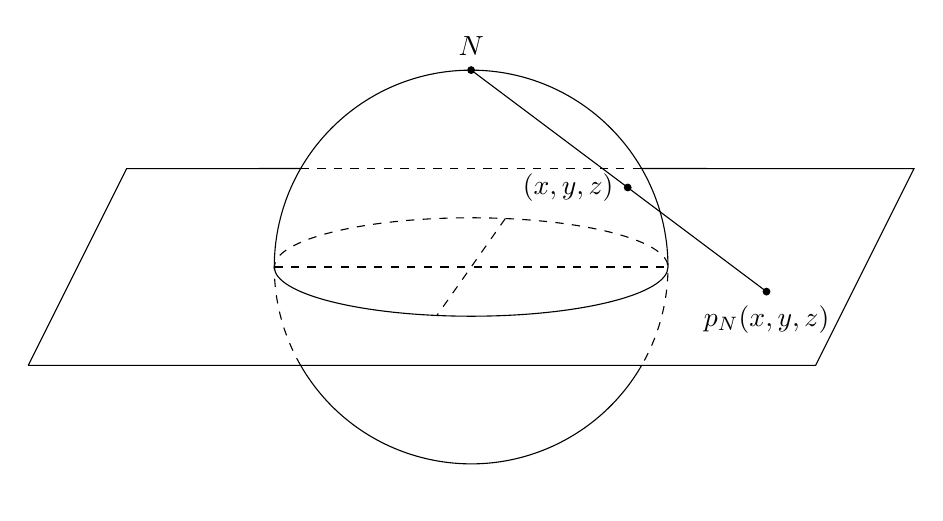
\begin{tikzpicture}[scale=1.25]
            \coordinate (A) at (3,-0.25);
            \coordinate (P) at (0,2);
      
            \draw (0:2cm)   arc[radius=2cm,start angle=0,end angle=180]
                  (210:2cm) arc[radius=2cm,start angle=210,end angle=330];
            \draw (180:2cm) arc[x radius=2cm, y radius=0.5cm, start angle=180,end angle=360];
      
            \draw [dashed] (210:2cm) 
                  arc[start angle=210,delta angle=-30,radius=2cm]
                  arc[start angle=180,delta angle=-180,x radius=2cm,y radius=0.5cm]
                  arc[start angle=0,delta angle=-30,radius=2cm];
      
            \draw [dashed] (80:2cm and 0.5cm) -- (260:2cm and 0.5cm);
            \draw [dashed] (150:2cm) coordinate(ul) -- (30:2cm) coordinate(ur);
      
            \draw (-4.5,-1) -- (3.5,-1) -- (4.5,1) -- (ur) (ul) -- (-3.5,1) -- (-4.5,-1);
      
            \draw (A) -- (P) coordinate[pos=0.47](B);
            \path (A) node[circle, fill, inner sep=1pt, label=below:{$ p_N(x,y,z) $}]{};
            \path (B) node[circle, fill, inner sep=1pt, label=left:{$ (x, y, z) $}]{};
            \path (P) node[circle, fill, inner sep=1pt, label=above:{$N$}]{};
            \draw [dashed] (-2,0) -- (2,0);
         \end{tikzpicture}
      \caption{Projection stéréographique de la sphère par rapport au pôle Nord}
   \end{figure*}
   On peut alors de manière analogue au cercle, trouver l'expression analytique des deux projections et montrer qu'elles munissent \( \mathbb{S}^2 \) d'une structure de variété différentielle.
\chapter{Espaces tangents dans \( \R^n \)}
On aimerait alors pouvoir généraliser la notion \textbf{d'espace tangent} à une courbe, surface ... lisse de \( \R^n \) à des variétés abstraites comme définies dans les deux premiers chapitres. Pour ce faire, il est fondamental de comprendre que les variétés ainsi définies ne sont \textbf{pas} des objets de \( \R^k \), donc la notion de vecteur tangent géométrique perd son sens.\<

L'approche fructueuse consiste alors à identifier \textbf{vecteurs} de \( \R^n \) et \textbf{dérivations} via la notion de dérivée directionnelle. On considère tout d'abord le cas de \( \R^n \), puis on généralise dans une variété quelconque.

\section{Notion de dérivation:}
Soit \(x \in \R^n\), on dira qu'un opérateur linéaire \( D: \mathcal{C}^\infty(\R^n) \longrightarrow \R \) est une \textbf{dérivation} en \( x \) si et seulement si elle vérifie la \textbf{règle de Leibniz} donnée par:
\[ 
   D(fg) = D(f)g(x) + f(x)D(g) 
\]
En particulier, les opérateurs de dérivées partielles d'une fonction lisse sont des dérivations. On peut aussi facilement montrer que si \( f \) est constant \( Df = 0 \) pour toute dérivation \( D \).
\section{Vecteurs géométriques:}
On considère l'espace \(\R^n_p := \left\{ p \right\} \times \left\{ v \; ; \; v \in \R^n \right\}\) des vecteurs \textbf{tangents géométriques}. On note ses éléments \( u_p \in \R^n_p\), alors on munit cet ensemble des opérations naturelles suivantes:
\begin{itemize}
   \item \(u_p + v_p = (p, u + v)\)
   \item \(\lambda u_p = (p, \lambda u)\)
\end{itemize}
Alors cet espace est naturellement muni d'une structure d'espace vectoriel de base canonique évidente \( (p, e_i)_{i \leq n} \).
\section{Espace tangent \( T\R^n_p \):}
On appelle alors \textbf{espace tangent} à \( \R^n_p \) l'ensemble \( T\R^n_p \) de toutes les dérivations de fonctions lisses définies sur \( \R^n_p \). On pose alors l'application suivante:
\[ 
   \begin{aligned}
      \Phi : \R^n_p &\longrightarrow T\R^n_p \\
      v_p &\longmapsto \sum_{i \leq n} v_i \partialD{}{x_i}\biggr|_p
   \end{aligned} 
\]
Alors on montre la propriété fondamentale qui est que \( \Phi \) est un \textbf{isomorphisme linéaire}. Ceci nous permet alors d'identifier vecteurs et dérivations, en outre, on en déduit une base de \( T\R^n_p \) qui est alors donnée par:
\[ 
   \Phi(e_i) = \partialD{}{x_i}\biggr|_p
\] 
\chapter{Espaces tangents sur une variété}
On généralise l'approche du chapitre précédent au cas des variétés, et on en déduit une définition de l'espace tangent en un point, intrinsèque et qui ne dépends pas des cartes. Dans toute la suite, on considèrera une fonction \( f : M \longrightarrow N \) point \( p \in M \), une carte \( \phi = (x_1, \ldots, x_n) \) et \( \psi = (y_1, \ldots, y_n) \) qui contiennent respectivement \( p \) et \( f(p) \)
\section{Espace tangent en un point:}
On définit une \textbf{dérivation} sur \( M \) comme un opérateur linéaire sur \( \mathcal{C}^\infty(M) \) qui vérifie la règle de Leibniz. On définit alors de manière analogue au cas euclidien \( TM_p \) comme l'ensemble des dérivations au point \( p \). C'est alors un espace vectoriel pour les lois usuelles.
\section{Différentielle}
On considère alors une application lisse \( f : M \longmapsto N \) et \( p \in M \). On définit alors la \textbf{différentielle} de l'application \( f \) en \( p \) par l'application suivante:
\[ 
   \begin{aligned}
      df_p : TM_p &\longrightarrow TN_{f(p)} \\
      D &\longmapsto \left( g \longmapsto D(g \circ f) \right)
   \end{aligned} 
\]
C'est moralement une application qui transporte les dérivations. On peut alors vérifier que cette application est bien définie et qu'elle vérifie les propriétés suivantes:
\begin{itemize}
   \item Elle est \textbf{linéaire}.
   \item Elle vérifie la \textbf{règle de la chaîne:} \( d(f \circ g)_p = df_{g(p)} \circ dg_p \)
   \item Si \( f \) est un \textbf{difféomorphisme}, alors \( \forall p \in M \; ; \; df_p \) est un \textbf{isomorphisme}.
\end{itemize}
On peut alors montrer que pour ces définitions, si on considère une carte \( (U, \phi) \) qui contient \( p \), alors c'est un \textbf{difféomorphisme} et donc on a l'isomorphisme suivant:
\[ 
   \begin{aligned}
      d\phi : TM_p &\longrightarrow T\R_{\phi(p)}^n
   \end{aligned} 
\]
On en déduis donc que \( TM_p \) est un espace vectoriel de dimension \( n \) et qu'une base  est donnée par:
\[ 
   \partialD{}{x_i}\biggr|_p := d\phi^{-1}\left( \partialD{}{x_i}\biggr|_{\phi(p)}\right) 
\]
Ce sont des dérivations dont l'action sur une fonction lisse\footnote[1]{Si \( f : M \longrightarrow N \) alors on peut aussi définir une action de ces dérivées partielles en composantes en notant \( f_j(p) = (\psi \circ f)_j(p) \) la \( j \)-ième composante de \( f \), et alors \( \partialD{}{x_i}\bigr|_p(f) := \left(\partialD{}{x_i}\bigr|_p(f_1), \ldots,  \partialD{}{x_i}\bigr|_p(f_n)\right) \)} \( f \) est définie par la dérivation partielle dans les coordonées locales:
\[ 
   \partialD{}{x_i}\biggr|_pf = \partialD{f \circ \phi^{-1}}{x_i}(\phi(p))
\]

\pagebreak
\section{Fibré tangent}
On cherche alors a globaliser la notion d'espace tangent et considérer \textbf{l'ensemble de tout les espaces tangents}. Ce point de vue est fructueux car il permettra de définir de manière simple la notion de champs de vecteurs sur une variété.\< 

On appelle cet ensemble le \textbf{fibré tangent} de \( M \) et il est défini par:
\[ 
   TM = \bigsqcup_{p \in M} TM_p = \bigcup_{p \in M} \{p\} \times TM_p
\]
\begin{figure}[h]
   \centering
   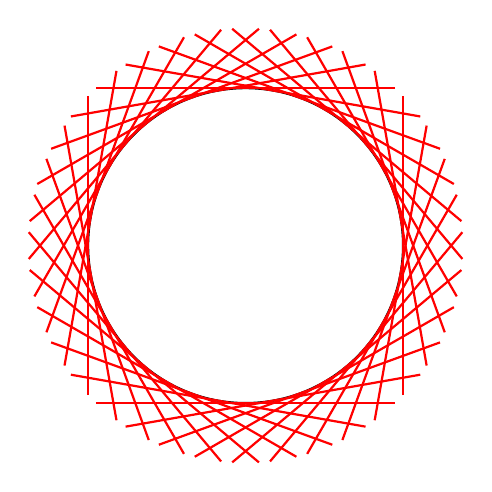
\begin{tikzpicture}
      % Dessiner le cercle
      \draw[thick] (0,0) circle (2);
      
      % Définir des points sur le cercle et leurs tangentes
      \foreach \angle in {10, 20, 30, 40, 50, 60, 70, 80, 90, 100, 110, 120, 130, 140, 150, 160, 170, 180, 190, 200, 210, 220, 230, 240, 250, 260, 270, 280, 290, 300, 310, 320, 330, 340, 350, 360} {
         % Calcul des coordonnées du point sur le cercle
         \pgfmathsetmacro\x{2*cos(\angle)}
         \pgfmathsetmacro\y{2*sin(\angle)}
          
         % Calcul du vecteur tangent (perpendiculaire au rayon)
         \pgfmathsetmacro\tx{-sin(\angle)}
         \pgfmathsetmacro\ty{cos(\angle)}
          
         % Tracer une droite tangentielle passant par le point
         \draw[red, thick] 
            ({\x - 1.9*\tx}, {\y - 1.9*\ty}) -- 
            ({\x + 1.9*\tx}, {\y + 1.9*\ty});
      }
   \end{tikzpicture}
   \caption{Fibré tangent du cercle \( \mathbb{S}^1 \)}
\end{figure}

Le fibré tangent hérite alors de plusieurs propriétés:
\begin{itemize}
   \item Une projection \( \pi : (p, v_p) \in TM \mapsto p\) appelée \textbf{trivialisation locale}.
   \item Une topologie définie par la préimage de celle ci.
\end{itemize}
De ces propriétés, on peut alors montrer que \( TM \) peut être muni d'une structure de \textbf{variété différentielle} de dimension \( 2n \). En effet on considère une carte \( (U, \phi) \) de \( M \), alors on pose:
\[ 
   \left(\pi^{-1}(U), (p, v_p) \mapsto (\phi(p), v_{p, 1}, \ldots, v_{p, n}) \right)
\]
Alors ceci définit une carte locale sur l'ouvert \(\pi^{-1}(U)\) et on peut alors montrer que l'ensemble des cartes ainsi construites forme bien un atlas sur \( TM \) (admis car non nécessaire pour la suite ?).\<

Un des intérêts de cette notion est qu'on peut alors identifier la différentielle comme une application globale sur les fibrés donnée par:
\[ 
   \begin{aligned}
      df : TM &\longrightarrow TN \\
      (p, v_p) &\longmapsto (f(p), df_p(v_p))
   \end{aligned} 
\]
\section{Champs de vecteurs}
On peut alors définir la notion de \textbf{champs de vecteurs} sur une variété \( M \) par la donnée d'une application lisse de la forme:
\[ 
   \begin{aligned}
      V : M &\longrightarrow TM \\
      p &\longmapsto (p, v_p)
   \end{aligned} 
\]
Où on identifiera \( V(p) \triangleq v_p \). Alors plus précisément, si on fixe \( p \in M \), alors en coordonées locales on a:
\[ 
   V(p) = \sum_{i = 1}^n V_i(p) \partialD{}{x_i}\biggr|_p
\]
\pagebreak
\section{Pushforward d'un champs de vecteurs}
Soit \( f : M \longrightarrow N \) une application lisse, l'utilité principale de la différentielle est de pouvoir transporter des vecteurs tangents à \( M \) sur des vecteurs tangents à \( N \), on peut alors se demander si on peut transporter un champs de vecteurs \( X : p \longrightarrow TM \) de la sorte, on peut toujours définir:
\[ 
   g_X : p \in M \longmapsto (f(p), df_p(X_p)) \in TN
\]
Mais ce n'est pas à proprement parler un champs de vecteurs sur \( N \) du fait du domaine de définition, néanmoins si \( f \) est une \textbf{difféomorphisme}, on peut définir le \textbf{pushforward} de \( X \) induit par \( f \) par:
\[ 
   f_*X : q \in N \longmapsto (q \; ; \; df_{f^{-1}(q)}(X_{f^{-1}(q)})) \in TN
\]
On obtient bien ainsi un champs de vecteurs sur \( N \).

\chapter{Espaces cotangents sur une variété}
On peut alors considérer naturellement l'espace dual à l'espace tangent en un point \( p \in M \) et on définit ainsi \textbf{l'espace cotangent} en un point. On notera une base de cet espace, dans des coordonées locales, par la famille \( (dx_i)_{i \leq n} \) qui vérifie par définition pour la base définie dans le chapitre précédent que:
\[ 
   dx_i\left(\partialD{}{x_j}\biggr|_p\right) = \delta_{i, j}
\]
\section{Fibré cotangent}
On peut alors de manière analogue globaliser la notion d'espace cotangent et considérer \textbf{l'ensemble de tout les espaces cotangents}. Ce point de vue est fructueux car il permettra de définir de manière simple la notion de champs de covecteurs, de formes différentielles et de manière générale d'étendre l'algèbre tensorielle aux variétés.\< 

On appelle cet ensemble le \textbf{fibré cotangent} de \( M \) et il est défini par:
\[ 
   TM^* = \bigsqcup_{p \in M} TM^*_p = \bigcup_{p \in M} \{p\} \times TM^*_p
\]
C'est, par définition du dual d'un fibré vectoriel\footnote[1]{Le dual du fibré, c'est le fibré des duals (:}, le dual de \( TM \). Aussi, il vérifie des propriétés analogues au fibré vectoriel et c'est aussi une variété de dimension \( 2n \).
\section{Identification de la différentielle à une forme:}
L'expression de la différentielle d'une fonction \( f : M \longrightarrow \R \) s'identifie à l'expression usuelle d'une différentielle, en effet, si \( v \in TM_p \), alors pour toute fonction lisse \( g : \R \longrightarrow \R \) on a:
\begin{align*}
   df_p(v)(g) &= \sum_{i=1}^n v_i df_p\left(\partialD{}{x_i}\biggr|_p\right)(g)\\
   &= \sum_{i=1}^n v_i \partialD{g \circ f}{x_i}(p)\\
   &= \sum_{i=1}^n v_i \partialD{g}{t}(f(t))\partialD{f}{x_i}(p)\\
   &= \left(\sum_{i=1}^n v_i \partialD{f}{x_i}(p)\partialD{}{t}\biggr|_{f(p)}\right)(g)
\end{align*}
Ceci étant vrai pour toute fonction lisse \( g \), on trouve l'expression suivante:
\[ 
   df_p(v) = \sum_{i=1}^n v_i \partialD{f}{x_i}(p)\partialD{}{t}\biggr|_{f(p)}
\]
Or, le vecteur de base \(\partialD{}{t}\) de \( T\R_{f(p)} \) s'identifie naturellement à la base canonique de \( \R \), on a aussi \( v_i = dx_i(v) \) donc on a l'identification naturelle suivante:
\[ 
   df_p(v) \triangleq \sum_{i=1}^n \partialD{f}{x_i}(p)dx_i(v)
\]
On remarque alors que \( df_p \in TM^*_p \), on peut donc identifier la différentielle d'une fonction scalaire évaluée en un point à un vecteur cotangent, ie une forme linéaire sur l'espace tangent.
\section{Identification de la différentielle dans le cas général:}
L'expression de la différentielle d'une fonction \( f : M \longrightarrow N \) s'identifie aussi à l'expression usuelle d'une différentielle, en effet, si \( v \in TM_p \), alors pour toute fonction lisse \( g : M \longrightarrow \R \)on a:
\begin{align*}
   df_p(v)(g) &= \sum_{i=1}^n v_i df_p\left(\partialD{}{x_i}\biggr|_p\right)(g)\\
   &= \sum_{i=1}^n v_i \partialD{g \circ f}{x_i}(p)\\
   &= \sum_{i=1}^n v_i \sum_{j=1}^m \partialD{g}{y_j}(f(p)) \partialD{f_j}{x_i}(p)\\
   &= \left(\sum_{i=1}^n\sum_{j=1}^m v_i \partialD{f_j}{x_i}(p)\partialD{}{y_j}\biggr|_{f(p)}\right)(g)
\end{align*}
Où ici \( f_j \) représente les coordonées locales de \( f \) au voisinage de \( f(p) \), ie \( f_j = (\psi \circ f)_j(p) \). Ceci étant vrai pour toute fonction lisse \( g \), on trouve l'expression suivante:
\[ 
   df_p(v) = \sum_{i=1}^n\sum_{j=1}^m v_i \partialD{f_j}{x_i}(p)\partialD{}{y_j}\biggr|_{f(p)}
\]
Or, le vecteur de base \(\partialD{}{y_j}\) de \( TN_{f(p)} \) s'identifiant naturellement au vecteur la base canonique de \( \R^n \), on a l'identification naturelle suivante:
\[ 
   df_p(v) \triangleq \sum_{i=1}^n \left( \partialD{f_1}{x_i}(p), \ldots, \partialD{f_m}{x_i}(p)\right)dx_i(v) = (df_{1, p}(v), \ldots, df_{m, p}(v))
\]
De manière analogue on peut aussi remarque que la matrice de la différentielle dans les cartes est alors donnée par la jacobienne associée.
\chapter{Formes différentielles sur une variété}
On peut alors définir la notion de \textbf{champs de covecteurs} sur une variété \( M \), ie la notion de 1-forme différentielle. Elle est définie par la donnée d'une application lisse de la forme:
\[ 
   \begin{aligned}
      \omega : M &\longrightarrow TM^* \\
      p &\longmapsto (p, \omega_p)
   \end{aligned} 
\]
Où on identifiera \( \omega(p) \) et \(\omega_p\). Alors plus précisément, si on fixe \( p \in M \), alors en coordonées locales on a:
\[ 
   \omega(p) = \sum_{i = 1}^n \omega_i(p) dx_i
\]
\section{Différentielles d'une fonction}
On remarque alors qu'un exemple remarquable de 1-forme différentielle est celui de la différentielle elle même d'une fonction \( f : M \longrightarrow \R \), en effet, on a expliqué plus haut que l'on peut identifier:
\[ 
   df_p \triangleq  \sum_{i=1}^n \partialD{f}{x_i}(p)dx_i
\]
\section{Formes différentielles de degré k}
Plus généralement, l'espace tangent \( TM_k \) est un espace vectoriel, donc on peut considèrer l'ensemble des \( k \)-tenseurs covariants sur celui-ci, qu'on notera \( \Lambda^k(TM_p^*) \), et de manière analogue aux constructions précédentes, on construit la \( k \)-ième puissance extérieur du fibré cotangent par:
\[ 
   \Lambda^k(TM^*) = \bigsqcup_{p \in M} \Lambda^k(TM_p^*) = \bigcup_{i \in M} \left\{ p \right\} \times \Lambda^k(TM_p^*) 
\]
Et finalement définir l'ensemble des \( k \)-formes différentielles, noté \( \Omega^k(M) \) comme l'ensemble des applications de la forme:
\[ 
   \begin{aligned}
      \omega : M &\longrightarrow \Lambda^k(TM^*)
   \end{aligned} 
\]
Qui, d'aprés le chapitre introductif sur l'algèbre tensorielle, s'écrivent dans la base locale sous la forme suivante:
\[ 
   \omega = \sum_{1 \leq i_1 < \ldots < i_k \leq n} \omega_{i_1, \ldots, i_k}(p) dx_{i_1} \wedge \ldots \wedge dx_{i_k}
\]
\section{Formes volumes}
On appelle \textbf{forme volume} sur \( M \) tout élément de \( \Omega^n(M) \) qui ne \textbf{s'annule pas}. On dira alors que \( M \) est \textbf{orientable}.

\pagebreak
\section{Evaluation d'un forme}
Une 1-forme différentielle \( \omega \) étant un champs de formes linéaires, si on fixe \( p \in M \), on peut alors évaluer cette forme en un champs de vecteurs \( X \), et cette opération est donnée par:
\[ 
   \omega(X) : p \longmapsto \omega_p(X_p)
\]
Alors, on peut exprimer cette évaluation en coordonées locales, ie si on a une forme différentielle d'ordre \( k \) et un champs de vecteurs de la forme suivante:
\[
   \omega(p) = \sum_{i \leq n} \omega_{i}(p) dx_{i} \quad\quad\quad\quad X = \sum_{i \leq n} x_i \partialD{}{x_i}\biggr|_{\phi(p)}
\]
Alors on a par définition de la base duale:
\begin{align*}
   \omega(X)(p) &=  \sum_{1 \leq i \leq n} \omega_{i}(p) dx_{i}\left(\sum_{j \leq n} x_j \partialD{}{x_j}\biggr|_{\phi(p)} \right)\\
   &=  \sum_{1 \leq i \leq n} \omega_{i}(p)x_i
\end{align*} 
Donc pour un point \( p \) fixé, une 1-forme est un objet qui prends un \textbf{champs de vecteurs} et retourne une \textbf{fonction} de \( p \). De manière analogue on peut généraliser et évaluer une \( k \)-forme sur \( k \) champs de vecteurs et obtenir une fonction.
\section{Dérivée extérieure locale}
En un point \( p \in M \), on peut alors définir l'opérateur de \textbf{dérivée extérieure} (au voisinage du point \( p \)) conformément au chapitre I par:
\[ 
   \begin{aligned}
      d_p^k : \Omega^k_p(M) &\longrightarrow \Omega^{k+1}_p(M) \\
      \omega &\longmapsto d \omega
   \end{aligned} 
\]
Où \( d \omega \) est défini encoordonées locales conformément à la définition usuelle par différentiation de la fonction coefficients:
\[ 
   d \omega_p = \sum_{1 \leq i_1 < \ldots < i_k \leq n} d\omega_{i_1, \ldots, i_k}(p) \wedge dx_{i_1} \wedge \ldots \wedge dx_{i_k}
\]
On peut alors faire une remarque sur cette définition, si \( f \) est une fonction lisse alors la différentielle \( df_p \) s'identifie bien à l'application de cet opérateur à \( f \) en tant que \( 0 \)-forme. En particulier si \( x_i \) est la fonction i-ème coordonée, alors ceci justifie la notation \( dx_i \) pour la base de l'espace cotangent.
\section{Dérivée extérieure globale}
On aimerait alors pouvoir définir cet opérateur globalement, comme dans le cas de \( \R^n \), on montre alors que cette définition locale ne dépends pas du choix de la carte et donc on peut définir cet opérateur globalement:
\[ 
   \begin{aligned}
      d^k : \Omega^k(M) &\longrightarrow \Omega^{k+1}(M) \\
      \omega &\longmapsto d \omega
   \end{aligned} 
\]
Et alors il vérifie toutes les propriétés de la dérivée extérieure de \( \R^n \).
\section{Pullback d'un champs de covecteurs}
Dans la section sur les champs de vecteurs, on a vu que la différentielle d'une application \( f : M \longrightarrow N \) permet de transporter ceux-ci par \textbf{pushforward}. On définit ici le concept dual (associé à l'adjoint de la différentielle) qui permet de transporter des champs de covecteurs dans le sens opposé.\<

Etant donnée une \( 1 \)-forme différentielle \( \omega \) sur \( N \), on peut alors \textbf{toujours} définir le \textbf{pullback} de \( \omega \) induit par \( f \) par:
\[ 
   f^*\omega : p \in M \longrightarrow (p, \omega_{f(p)} \circ df_p) \in TM^*
\]
Alors c'est bien une forme différentielle sur \( M \). 
\section{Pullback d'une forme différentielle}
De manière générale pour une \( k \)-forme on définit en composant par un \( k \)-uplet de différentielles de \( f \):
\[ 
   f^*\omega : p \in M \longrightarrow (p, \omega_{f(p)} \circ (df_p, \ldots, df_p)) \in TM^*
\]
\section{Propriétés du pullback}
Le pullback d'une \( k \)-forme sera un des outils principaux pour construire la théorie de l'intégration sur une variété. On a donc besoin d'étudier ses propriétés, alors on peut montrer qu'on a:
\begin{itemize}
   \item Le pullback est \textbf{linéaire}.
   \item Le pullback respecte le \textbf{produit extérieur}:
   \[ 
      f^*(\omega \wedge \eta) = f^*(\omega) \wedge f^*(\eta)
   \]
   \item Le pullback respecte la \textbf{dérivée extérieure}:
   \[ 
      f^*(d\omega) = d(f^*\omega)
   \]
\end{itemize}
\chapter{Orientation d'une variété à bord}
Dans le troisième chapitre, on a définit la notion de variété à bord, puis par la suite celle de forme volume qui définit une orientation sur une variété \( M \). On se pose alors la question suivante:
\begin{center}
   \textit{Est-il possible de construire une orientation sur \( \partial M \) étant donnée une orientation sur \( M \) ?}
\end{center}
On considère par la suite une variété à bord de dimension \( n \)